\chapter{Effectiveness of QUBO splitting}\label{sec:qsplitres}

The following chapter analyzes the effectiveness of \texttt{QSplitSampler} when applied to ``real'' problems.

The analysis compares \texttt{QSplitSampler} with D-Wave's solver that directly utilizes the QPU, namely \texttt{QPUSampler}.
The data collected focuses on:
\begin{itemize}
    \item The quality of the solution produced, specifically how close the assignment is to the global optimum;
    \item The time required for the resolution, considering both time spent on the QPU and CPU.
\end{itemize}

Section \ref{sec:maxcut} examines a specific instance of the Maximum-Cut Problem (MCP).
The selected instance can be easily visualised and has some desirable features for evaluating the performance of \texttt{QSplitSampler} under ``adverse'' conditions.

Section \ref{sec:qsplittest} analyzes a series of randomly generated problems to evaluate not only the solution quality but, more importantly, the time advantage of \texttt{QSplitSampler} compared to \texttt{QPUSampler} by assessing whether increased QPU usage results in a shorter overall time to compute the solution.

\section{Test case: Maximum-Cut Problem}\label{sec:maxcut}

To evaluate \texttt{QSplitSampler} effectiveness it is natural to set a controlled environment, as opposed to the real scenario provided by sentiment analysis applications.
The real scenario selected is represented by the solution to instances of MCP, reduced to QUBO. 

Motivations to choose MCP are:
\begin{itemize}
    \item It is straightforward to manually construct problems with a specified number of edges and nodes;
    \item It is a problem that can be reformulated easily in QUBO form;
    \item It exhibits symmetric solutions, meaning that the assignment of binary variables or their complementary assignment yields the same objective function value.
    Therefore, the optimal solution to MCP will never be unique, as there will always be at least two optimal assignments.
\end{itemize}

\subsection{Maximum-Cut}

MCP involves dividing the vertices of a graph into two subsets, $S$ and $T$, such that the number of edges between nodes in $S$ and nodes in $T$ is maximized.

Consider a graph like the one in Figure \ref{fig:maxcut}. 
Subset $S$ consists of the white nodes, and subset $T$ consists of the black nodes. 
Figure \ref{fig:maxcutset} highlights all and only the edges between $S$ and $T$.

\begin{figure}[H]
    \centering
    \begin{subfigure}[b]{0.48\textwidth}
        \centering
        \begin{tikzpicture}
            \node[circle, fill=white, draw=black, inner sep=2pt, label=above:$A$] (A) at (0,2) {};
            \node[circle, fill=black, draw=black, inner sep=2pt, label=above:$B$] (B) at (2,2) {};
            \node[circle, fill=white, draw=black, inner sep=2pt, label=below:$C$] (C) at (2,0) {};
            \node[circle, fill=black, draw=black, inner sep=2pt, label=below:$D$] (D) at (0,0) {};
            \node[circle, fill=black, draw=black, inner sep=2pt, label=above:$E$] (E) at (-1.5,1) {};
            
            \draw[red, thick] (A) -- (B);
            \draw[red, thick] (B) -- (C);
            \draw[red, thick] (C) -- (D);
            \draw[red, thick] (D) -- (A);
            \draw[red, thick] (A) -- (E);
            \draw[black, thick] (E) -- (D);
        
            \draw[blue, thick] ($(A)+(0.75,0.5)$) -- ($(C)+(0.75,-0.75)$) -- ($(C)+(-0.75,-0.75)$) -- ($(A)+(-0.75,0.5)$);
        \end{tikzpicture}
        \caption{Maximum-Cut example graph.}
        \label{fig:maxcut}
    \end{subfigure}
    \hfill
    \begin{subfigure}[b]{0.48\textwidth}
        \centering
        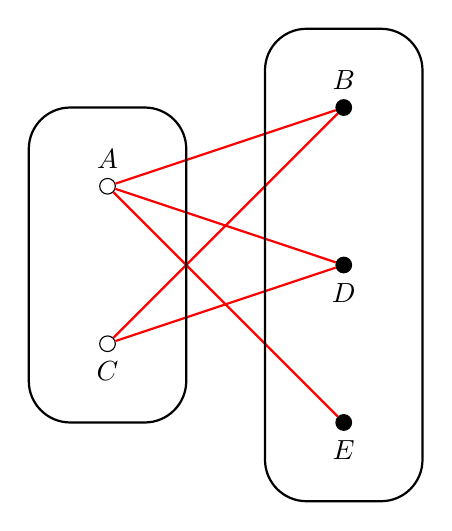
\begin{tikzpicture}
            \node[circle, fill=white, draw=black, inner sep=2pt, label=above:$A$] (A) at (0,3) {};
            \node[circle, fill=white, draw=black, inner sep=2pt, label=below:$C$] (C) at (0,1) {};
            
            \node[circle, fill=black, draw=black, inner sep=2pt, label=above:$B$] (B) at (3,4) {};
            \node[circle, fill=black, draw=black, inner sep=2pt, label=below:$D$] (D) at (3,2) {};
            \node[circle, fill=black, draw=black, inner sep=2pt, label=below:$E$] (E) at (3,0) {};
            
            \draw[red, thick] (A) -- (B);
            \draw[red, thick] (A) -- (E);
            \draw[red, thick] (A) -- (D);
            \draw[red, thick] (C) -- (B);
            \draw[red, thick] (C) -- (D);
            
            \draw[black, thick, rounded corners=15pt] (-1,0) rectangle (1,4);
            \draw[black, thick, rounded corners=15pt] (2,-1) rectangle (4,5);
        \end{tikzpicture}
        \caption{Rearranged graph in $S$ and $T$.}
        \label{fig:maxcutset}
    \end{subfigure}
    \caption{Maximum-Cut (a) and subdivision into subsets (b).}
\end{figure}

\paragraph{Desired Characteristics} In the case illustrated in Figure \ref{fig:maxcut}, it is easily verifiable that it is impossible to find an assignment of $S$ and $T$ that produces more than five edges.

However, the solution is not unique. 
Associating $1$ with the white nodes and $0$ with the black nodes, two five-edge solutions are: 
\begin{itemize}
    \item $\{A=1,B=0,C=1,D=0,E=0\}$,
    \item $\{A=0,B=1,C=0,D=1,E=1\}$.
\end{itemize}

The non-uniqueness of the solution presents a challenge during the optimization process, as different sections of the problem might guide towards complementary assignments, leading to inconsistent aggregated results when, recalling Section \ref{sec:split}, a QUBO problem is splitted, possibly recursively, into smaller instances.

\subsection{Results}

\texttt{QSplitSampler} was configured to solve problems using \texttt{QPUSampler} that only consider two variables. 
Since the initial problem size consists of eight variables, the submatrices considered for direct resolution have a size equal to $\frac{2^2}{8^2} = \frac{1}{16}$ of the original problem.

In this case, partitioning is unnecessary, as the QPU can directly solve problems of this size. 
The utility of this experiment lies in providing an initial measure of error.

In particular, the instance of MCP under consideration is represented in Figure \ref{fig:maxcut_test}.
The graph represents a problem with eight nodes, corresponding to eight binary variables.

\begin{figure}[H]
    \centering
    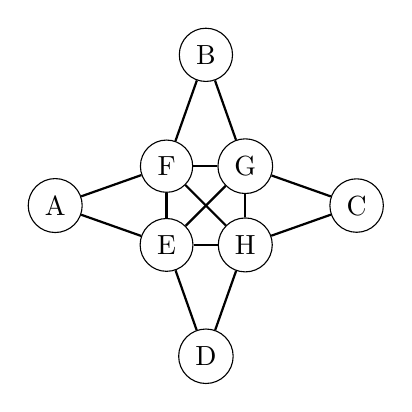
\begin{tikzpicture}
        \node[circle, draw=black] (A) at (0,1.914) {A};
        \node[circle, draw=black] (B) at (1.914,3.828) {B};
        \node[circle, draw=black] (C) at (3.828,1.914) {C};
        \node[circle, draw=black] (D) at (1.914,0) {D};
        \node[circle, draw=black] (E) at (1.414,1.414) {E};
        \node[circle, draw=black] (F) at (1.414,2.414) {F};
        \node[circle, draw=black] (G) at (2.414,2.414) {G};
        \node[circle, draw=black] (H) at (2.414,1.414) {H};

        \draw[black, thick] (A) -- (E);
        \draw[black, thick] (A) -- (F);
        \draw[black, thick] (B) -- (F);
        \draw[black, thick] (B) -- (G);
        \draw[black, thick] (C) -- (G);
        \draw[black, thick] (C) -- (H);
        \draw[black, thick] (D) -- (H);
        \draw[black, thick] (D) -- (E);
        \draw[black, thick] (E) -- (F);
        \draw[black, thick] (E) -- (H);
        \draw[black, thick] (E) -- (G);
        \draw[black, thick] (F) -- (G);
        \draw[black, thick] (F) -- (H);
        \draw[black, thick] (H) -- (G);
    \end{tikzpicture}
    \caption{Graph used to test Maximum-Cut.}
    \label{fig:maxcut_test}
\end{figure}

Following the examples provided by D-Wave itself \cite{maxcut-dwave}, it is possible to convert the graph in Figure \ref{fig:maxcut_test} into a QUBO formulation, resulting in the upper triangular matrix shown in the matrix \eqref{eq:maxcutQUBO}.

\begin{equation}
    \begin{array}{c|*{8}{c}}
          & A  & B  & C  & D  & E  & F  & G  & H  \\
        \hline
        A & -2 & 0  & 0  & 0  & 2  & 2  & 0  & 0  \\
        B &    & -2 & 0  & 0  & 0  & 2  & 2  & 0  \\
        C &    &    & -2 & 0  & 0  & 0  & 2  & 2  \\
        D &    &    &    & -2 & 2  & 0  & 0  & 2  \\
        E &    &    &    &    & -5 & 2  & 2  & 2  \\
        F &    &    &    &    &    & -5 & 2  & 2  \\
        G &    &    &    &    &    &    & -5 & 2  \\
        H &    &    &    &    &    &    &    & -5 \\
    \end{array}
    \label{eq:maxcutQUBO}
\end{equation}

Solving the problem \eqref{eq:maxcutQUBO} yields the results given in Table \ref{tab:maxcut}.

\begin{table}[H]
    \centering
    \begin{tabular}{cccc}
        \toprule
        \multicolumn{2}{c}{\texttt{QSplitSampler}} & \multicolumn{2}{c}{\texttt{QPUSampler}} \\
        Time (s) & Solution & Time (s) & Solution \\
        \midrule
        18.15 & 0.8 & 5.02 & 0        
    \end{tabular}
    \caption{\texttt{QSplitSampler} executed on \eqref{eq:maxcutQUBO}.}
    \label{tab:maxcut}
\end{table}

The time required to process the problem is expressed in seconds and includes the following components: 
\begin{itemize} 
    \item Processing on the CPU, which, in the case of a direct solution, consists only of initializing the data structure; 
    \item Network transfer, to send the problem to quantum solvers;
    \item Processing on the QPU, to produce the solution. 
\end{itemize}

The solution is presented by normalizing the values within the range $[0, 1]$. 
Since these are minimization problems, $0$ corresponds to the optimal solution.

\paragraph{Time Analysis} The time required to solve MCP on the graph in Figure \ref{fig:maxcut_test} with \texttt{QSplitSampler} is 3.6 times greater than that of a direct resolution. 
In detail, three main components can be identified that contribute to the time spent on classical machines:
\begin{itemize}
    \item Calculation of the minor embedding;
    \item Partitioning algorithm and aggregation of the subproblems;
    \item Time required to send the subproblems generated to \texttt{QPUSampler}.
\end{itemize}
The last of these components represents the dominant factor that causes \texttt{QSplitSampler} to perform worse than \texttt{QPUSampler} for small-sized problems.
Since, it is necessary to transmit the data to D-Wave's cloud infrastructure, wait for processing, and then forward the result, this computational overhead might become marginal for instances where quantum acceleration is substantial, but it significantly impacts the resolution of ``small'' problems.

\paragraph{Quality of Results} From a performance perspective, \texttt{QSplitSampler} produced results that were significantly worse compared to direct resolution. 
However, it is important to contextualize these results.

\texttt{QSplitSampler} provided a response of $0.8$, a value closer to the maximum assignment than to the minimum. 
For the tests conducted, this represents an upper bound on the error made in producing a solution. 
The poor quality of the response could be due to multiple optimal solutions, all equivalent from an algorithmic standpoint but leading to final assignments that are inconsistent with the original problem.

\section{Extensive testing}\label{sec:qsplittest}

To evaluate the performance of \texttt{QSplitSampler} in a broader context than that described in Section \ref{sec:maxcut}, random problems were generated using D-Wave's libraries. 
The problems considered represent complete graphs, and while they do not represent SVMs, they preserve their structure and information density.

Working with complete graphs increases the likelihood of having multiple optimal assignments. 
Intuitively, this occurs because the problem has more data to combine to converge to the same objective function value.

\subsection{64 and 128 Variables Problems}\label{sec:multivar}

Using D-Wave's libraries to generate complete graphs, problems with $64$ and $128$ variables were solved, with the results reported in Tables \ref{tab:64var} and \ref{tab:128var}, respectively.

The table columns provide the following information, with all times expressed in seconds: 
\begin{enumerate}
    \item \texttt{QSplitSampler}
    \begin{enumerate}
        \item \emph{Cut Dim}: Number of variables handled by the subproblem sent directly to \texttt{QPUSampler};
        \item \emph{CPU \& QPU time}: Represented as \emph{CPU time - QPU time};
        \item \emph{Solution};
    \end{enumerate}
    \item \texttt{QPUSampler}
    \begin{enumerate}
        \item \emph{CPU \& QPU time}: Represented as \emph{CPU time - QPU time};
        \item \emph{Solution}.
    \end{enumerate}
\end{enumerate}

\begin{itemize}
    \item \emph{CPU time}: The time required by \texttt{QSplitSampler} to produce a solution, which includes:
    \begin{itemize}
        \item The time take for minor embedding computation;
        \item The time for network transfer to D-Wave's cloud infrastructure;
        \item The time spent on classical architecture processing (partition and aggregation of results).
    \end{itemize}
    \item \emph{QPU time}: The time spent on the QPU;
    \item \emph{Solution} is the value of the best solution, normalized to $[0, 1]$.
\end{itemize}

\subsubsection{Results}

Referring to the first row of Table \ref{tab:64var}, it can be observed that the total time required to provide the solution using \texttt{QSplitSampler} is approximately seven times greater than that required by \texttt{QPUSampler}.
The increased time is due to the number of subproblems processed, a topic that will be discussed in detail in Section \ref{sec:subproblemcount}.

As well as the time spent on the CPU, the time spent on the QPU increases significantly, by a factor of 16.5, where \texttt{QSplitSampler} takes 0.33 seconds compared to 0.02 seconds for \texttt{QPUSampler}.

However, the quality of the solution produced is unacceptable; while \texttt{QPUSampler} reaches the global optimum, \texttt{QSplitSampler} deviates significantly, yielding a value of 0.45.

\begin{table}[H]
    \centering
    \begin{tabular}{ccc|cc}
        \toprule
        \multicolumn{3}{c}{\texttt{QSplitSampler}} & \multicolumn{2}{c}{\texttt{QPUSampler}} \\
        Cut Dim & CPU \& QPU time & Solution & CPU \& QPU time & Solution \\
        \midrule
        2 & 154.23 - 0.33 & 0.45 & 22.06 - 0.02 & 0 \\
        4 & 73.76 - 0.25 & 0.42 & 21.41 - 0.02 & 0 \\
        8 & 40.51 - 0.17 & 0.43 & 36.54 - 0.02 & 0 \\
        16 & 24.6 - 0.10 & 0.42 & 37.87 - 0.02 & 0 \\
        32 & 20.68 - 0.05 & 0.33 & 16.67 - 0.02 & 0 \\
        \bottomrule
    \end{tabular}
    \caption{Results for problems with 64 variables.}
    \label{tab:64var}
\end{table}

\begin{table}[H]
    \centering
    \begin{tabular}{ccc|cc}
        \toprule
        \multicolumn{3}{c}{\texttt{QSplitSampler}} & \multicolumn{2}{c}{\texttt{QPUSampler}} \\
        Cut Dim & CPU \& QPU time & Solution & CPU \& QPU time & Solution \\
        \midrule
        2 & 414.42 - 0.45 & 0.36 & 144.29 - 0.02 & 0 \\
        4 & 169.13 - 0.35 & 0.47 & 183.23 - 0.02 & 0 \\
        8 & 95.89 - 0.25 & 0.5 & 168.34 - 0.02 & 0 \\
        16 & 63.83 - 0.17 & 0.52 & 106.02 - 0.02 & 0 \\
        32 & 45.42 - 0.1 & 0.42 & 143.97 - 0.02 & 0 \\
        \bottomrule
    \end{tabular}
    \caption{Results for problems with 128 variables.}
    \label{tab:128var}
\end{table}

In both tables, the quality of the solution produced deviates significantly from the optimum, deteriorating between 25\% and 50\%. 
Furthermore, the lower limit of the error committed seems to increase as the problem size increases, stabilising at around 35\%.

Despite the suboptimal results, \texttt{QSplitSampler} maintains the desired behaviour regarding QPU usage. 
All reported values exceed 0.1 seconds, three times higher than the use of D-Wave's hybrid solver (Section \ref{sec:qpuusage}) for significantly larger problems.

However, despite the significant increase in the quantum component used to find the solution, the time required to transmit all the subproblems and aggregate the results remains dominant.

Based on the results obtained, the following key considerations emerge: 
\begin{itemize} 
    \item The effectiveness of maximizing QPU usage as a resolution strategy; 
    \item The evident increase in solution time as \emph{cut dim} decreases. 
\end{itemize}

\paragraph{Performance} Although no clear relationship emerges between the parameters \texttt{QSplitSampler} and the quality of the solution produced, it is evident that an error of at least 25\% for small-sized problems is not acceptable. 
The poor performance is likely due to the search for complementary assignments, a case which is not currently addressed during execution but may warrant further analysis.

\paragraph{Solving Time} The increase in solution time as \emph{cut dim} decreases is considerable, raising the question of where most of the time is spent during execution. 
Understanding the bottleneck of the current implementation may allow for the development of a second, potentially more efficient version.

\subsection{Subproblem Count}\label{sec:subproblemcount}

The methods used for subdivision and aggregation of subproblems are efficient enough not to have a significant impact on execution.

Likewise, the time required for transmission to the cloud infrastructure should not be so high as to slow down execution. 
However, how many subproblems are transferred remains to be verified. 
Although a single transmission may be negligible, extensive use of network resources could justify the observed behaviour.

Imagine an example problem like the one in Figure \ref{fig:exstart}.

\begin{figure}[H]
    \centering
    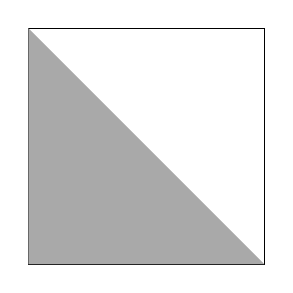
\begin{tikzpicture}
        \draw (0,0) rectangle (3,3);
        \fill[gray!90, opacity=0.75] (3, 0) -- (0, 0) -- (0, 3) -- cycle;
    \end{tikzpicture}
    \caption{General QUBO problem.}
    \label{fig:exstart}
\end{figure}

Once partitioned by the splitting operation, the result is what is presented in Figure \ref{fig:exsplit}, where of the four subproblems, only three require a solution to be aggregated.

\begin{figure}[H]
    \centering
    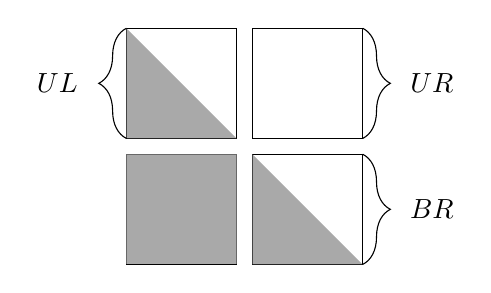
\begin{tikzpicture}
        \draw (0,0) rectangle (1.4,1.4);
        \draw (1.6,1.6) rectangle (3,3);
        \draw (0,1.6) rectangle (1.4,3);
        \draw (1.6,0) rectangle (3,1.4);
        \fill[gray!90, opacity=0.75] (0,0) -- (0,1.4) -- (1.4,1.4) -- (1.4,0);
        \fill[gray!90, opacity=0.75] (0,1.6) -- (0,3) -- (1.4,1.6) -- cycle;
        \fill[gray!90, opacity=0.75] (1.6,0) -- (3,0) -- (1.6,1.4) -- cycle;

        \draw[decorate,decoration={brace,amplitude=10pt}] (0,1.6) -- (0,3) node [black,midway,xshift=-25pt] {$\operatorname{UL}$};
        \draw[decorate,decoration={brace,amplitude=10pt,mirror}] (3,1.6) -- (3,3) node [black,midway,xshift=25pt] {$\operatorname{UR}$};
        \draw[decorate,decoration={brace,amplitude=10pt,mirror}] (3,0) -- (3,1.4) node [black,midway,xshift=25pt] {$\operatorname{BR}$};
    \end{tikzpicture}
    \caption{One step split.}
    \label{fig:exsplit}
\end{figure}

For each step of the recursive partition, three new problems are generated, which in turn can be further partitioned.

So, to handle a problem with $2^a$ variables by sending subproblems of size $2^b$ to the QPU, where $a \geq b$, means transmitting a total of $3^{a-b}$ subproblems to \texttt{QPUSampler}, where 3 is the number of subproblems generated by a single execution of the split step and $(a-b)$ is the number of recursive calls of \texttt{QSplitSampler}.

This calculation considers only the number of subproblems sent to the QPU by the splitting procedure. 
Conflict resolution also generates new subproblems, but their number grows linearly with the recursive calls of \texttt{QSplitSampler}. For this reason, its contribution may be disregarded as the growth in the number of subproblems is dominated by the base-3 exponentiation.

Thus, for a problem with $128$ variables ($2^7$) and a \emph{cut dim} of $2$, the number of subproblems transmitted is at least: $3^{7-1}=3^6=729$.

Although \texttt{QSplitSampler} allows for handling problems larger than the QPU limits (Section \ref{sec:qpu-res}), the proposed methodology is insufficient for solving problems of the size discussed in Section \ref{sec:qsvm-res}. 
The version of SVM used generates a problem with $32,768$ ($2^{15}$) variables, calculated according to Equation \eqref{eq:nodesnum}. 
Even assuming a \emph{cut dim} of $64$ ($2^6$), the number of problems to be sent to the QPU would be at least $3^{15-6}=3^9=19,683$.
